\documentclass[12pt,phd,times]{pkmthesis}

\usepackage{amsmath,epsfig,graphicx,setspace,url,float}
\usepackage{pstricks,colortab,pifont}
\usepackage{lscape,multicol,multirow,longtable,subfigure}
\usepackage{cite, bm}   
\usepackage{geometry}
\usepackage{array}
\usepackage{algorithm}
\usepackage{multirow}
\usepackage{tabularx}
\usepackage{graphicx} 
\usepackage{subcaption}
\usepackage{booktabs}% Due to this hyberref will not work for references (PKM on 07/07/08)
\usepackage[english]{babel}
\usepackage[small,bf]{caption}              % Added on 26/08/08
%\usepackage{slashbox} 
\usepackage{csquotes}  
\usepackage{threeparttable}
%\usepackage{adjustbox}                    % Added on 24/10/08 (Senthil)
\setlength{\textfloatsep}{1cm}              % Spacing b/w  float and text (PKM 01/11/08)
%..........................................................................................................................................
\normalem                                   % Added on 01/07/08 to avoid underline in the references
\setlength{\abovecaptionskip}{8pt}          % Added on 08/07/08
\setlength{\belowcaptionskip}{8pt}          % Added on 08/07/08
%..........................................................................................................................................
\usepackage{hyperref}
\usepackage{extra_functions}
%%*************************************************  MARGINS  ************************************************
% FOR SINGLE SIDE
%\hoffset 0in
%\voffset 0in
%\oddsidemargin 0.40cm
%\evensidemargin 0.55cm
%\marginparsep 0in
%\topmargin -0.25cm
%\textwidth 17cm
%\textheight 23.5cm
%\footskip 1.5cm

% FOR DOUBLE SIDE (03/09/08)
\hoffset 0in
\voffset 0in
\evensidemargin -0.4in
\oddsidemargin
 0.2cm
 \marginparsep 0in
 \topmargin 0.25cm
 \textwidth 17cm
\textheight 22.5cm
\footskip 1.5cm


%*************************************************************************************************************

\usepackage{fancyhdr}
\pagestyle{fancy}

%*************************************************************************************************************

\renewcommand{\chaptermark}[1]{\markboth{\thechapter.\ #1}{}}
\renewcommand{\sectionmark}[1]{\markright{\thesection\ #1}}

%\fancyhf{} \fancyhead[LE]{\bfseries\nouppercase{\leftmark}}
%\fancyhead[RO]{\bfseries\nouppercase{\rightmark}}

%*************************************************************************************************************
% HEADER & FOOTER HEADINGS  %PKM 04/07/08
%*************************************************************************************************************

\renewcommand{\headrulewidth}{0.5pt}
\renewcommand{\footrulewidth}{0.5pt}
\addtolength{\headheight}{2pt} % make space for the rule

%*************************************************************************************************************

\fancypagestyle{plain}{%
   \fancyhead{} % get rid of headers
   \renewcommand{\headrulewidth}{0pt} % and the line
   \renewcommand{\footrulewidth}{0pt}
}

%*************************************************************************************************************

\fancypagestyle{blank}{%
   \fancyhf{} % get rid of headers and footers
   \renewcommand{\headrulewidth}{0pt} % and the line
   \renewcommand{\footrulewidth}{0pt}
}

%*************************************************************************************************************

\fancypagestyle{abstract}{%
   \fancyhead{}
   \renewcommand{\headrulewidth}{0pt}
   \renewcommand{\footrulewidth}{0.5pt}
}

%*************************************************************************************************************

\fancypagestyle{document}{%
    \fancyhf{} \fancyhead[LE]{\bfseries\nouppercase{\leftmark}}
    \fancyhead[RO]{\bfseries\nouppercase{\rightmark}}
    \fancyfoot[LE,RO]{\bfseries\thepage}
    \renewcommand{\headrulewidth}{0.5pt}
    \renewcommand{\footrulewidth}{0.5pt}
    \addtolength{\headheight}{2pt} % make space for the rule
}

%*************************************************************************************************************
% SUBSECTION DEPTH  PKM on 05/07/08

\setcounter{secnumdepth} {5}
\setcounter{tocdepth} {5}
%\renewcommand{\thesubsubsection}{\thesubsection.\Alph{subsubsection}}   % (10/07/08- To remove Alpha number on subsubsubsection)

%*************************************************************************************************************
%\renewcommand{\subfigtopskip}{0.3 cm}
%\renewcommand{\subfigbottomskip}{0.2 cm}
%\renewcommand{\subfigcapskip}{0.3 cm}
%\renewcommand{\subfigcapmargin}{0.2 cm}

%*************************************************************************************************************
% PAGE SIZE & HYBERLINKS - PKM on 05/07/08

\hypersetup{     a4paper=true,
                 bookmarks,
                 bookmarksopen = true,  %false (18/07/08)
                 bookmarksnumbered = true,
                 breaklinks = true,
                 linktocpage,
                 pagebackref,
                 colorlinks = false,   %true (18/07/08)
                 linkcolor = blue,
                 urlcolor  = blue,
                 citecolor = red,
                 anchorcolor = green,
                 hyperindex = true,
                 linktocpage,
                 pagebackref,
                 hyperfigures,
                 pdftitle={SPEECH ENHANCEMENT},
                 pdfauthor={PKM},
                 pdfsubject={FINAL REPORT},
                 pdfcreator={ACROBAT 9 PROFESSIONAL},
                 pdfkeywords={This PDF is created with ACROBAT PROFESSIONAL 9 with PDFVERSION 1.5}}

%*************************************************************************************************************
           % Modified on 06/07/08, 10/07/08, 15/07/08
%%*************************************************  MARGINS  ************************************************
\hoffset 0in
\voffset 0in
%\oddsidemargin 0.40cm
\oddsidemargin 0.40cm
\evensidemargin 0.55cm
\marginparsep 0in
\topmargin -0.25cm
\textwidth 17cm
\textheight 23.5cm
\footskip 1.5cm

%*************************************************************************************************************

\usepackage{fancyhdr}
\pagestyle{fancy}

%*************************************************************************************************************

\renewcommand{\chaptermark}[1]{\markboth{\thechapter.\ #1}{}}
\renewcommand{\sectionmark}[1]{\markright{\thesection\ #1}}

%\fancyhf{} \fancyhead[LE]{\bfseries\nouppercase{\leftmark}}
%\fancyhead[RO]{\bfseries\nouppercase{\rightmark}}

%*************************************************************************************************************
% HEADER & FOOTER HEADINGS  %PKM 04/07/08
%*************************************************************************************************************

\renewcommand{\headrulewidth}{0.5pt}
\renewcommand{\footrulewidth}{0.5pt}
\addtolength{\headheight}{2pt} % make space for the rule

%*************************************************************************************************************

\fancypagestyle{plain}{%
   \fancyhead{} % get rid of headers
   \renewcommand{\headrulewidth}{0pt} % and the line
   \renewcommand{\footrulewidth}{0pt}
}

%*************************************************************************************************************

\fancypagestyle{blank}{%
   \fancyhf{} % get rid of headers and footers
   \renewcommand{\headrulewidth}{0pt} % and the line
   \renewcommand{\footrulewidth}{0pt}
}

%*************************************************************************************************************

\fancypagestyle{abstract}{%
   \fancyhead{}
   \renewcommand{\headrulewidth}{0pt}
   \renewcommand{\footrulewidth}{0.5pt}
}

%*************************************************************************************************************

\fancypagestyle{document}{%
	\fancyhf{} \fancyhead[LE]{\bfseries\nouppercase{\leftmark}}
	\fancyhead[RO]{\bfseries\nouppercase{\rightmark}}
	\fancyfoot[LE,RO]{\bfseries\thepage}
	\renewcommand{\headrulewidth}{0.5pt}
	\renewcommand{\footrulewidth}{0.5pt}
	\addtolength{\headheight}{2pt} % make space for the rule
}

%*************************************************************************************************************
% SUBSECTION DEPTH  PKM on 05/07/08

\setcounter{secnumdepth} {5}
\setcounter{tocdepth} {5}
%\renewcommand{\thesubsubsection}{\thesubsection.\Alph{subsubsection}}   % (PKM 10/07/08- To remove Alpha number on subsubsubsection)

%*************************************************************************************************************
%\renewcommand{\subfigtopskip}{0.3 cm}
%\renewcommand{\subfigbottomskip}{0.2 cm}
%\renewcommand{\subfigcapskip}{0.3 cm}
%\renewcommand{\subfigcapmargin}{0.2 cm}

%*************************************************************************************************************
% PAGE SIZE & HYBERLINKS PKM on 05/07/08

\hypersetup{     a4paper=true,
                 bookmarks,
                 bookmarksopen = true,  %false (18/07/08)
                 bookmarksnumbered = true,
                 breaklinks = true,
                 linktocpage,
                 pagebackref,
                 colorlinks = false,   %true (18/07/08)
                 linkcolor = blue,
                 urlcolor  = blue,
                 citecolor = red,
                 anchorcolor = green,
                 hyperindex = true,
                 linktocpage,
                 pagebackref,
                 hyperfigures,
                 pdftitle={SPEECH ENHANCEMENT},
                 pdfauthor={PKM},
                 pdfsubject={FINAL REPORT},
                 pdfcreator={ACROBAT 9 PROFESSIONAL},
                 pdfkeywords={This PDF is created with ACROBAT PROFESSIONAL 9 with PDFVERSION 1.5}}

%*************************************************************************************************************


       % For Single Sided Document 
%*************************************************  MARGINS  ************************************************
\hoffset 0in
\voffset 0in
%\oddsidemargin 0.40cm
\oddsidemargin -0cm
\evensidemargin -0cm
\marginparsep 0in
\topmargin -0.25cm
\textwidth 16cm
\textheight 23.5cm
\footskip 1.5cm

%*************************************************************************************************************

\usepackage{fancyhdr}
\pagestyle{fancy}

%*************************************************************************************************************

\renewcommand{\chaptermark}[1]{\markboth{\thechapter.\ #1}{}}
\renewcommand{\sectionmark}[1]{\markright{\thesection\ #1}}

%\fancyhf{} \fancyhead[LE]{\bfseries\nouppercase{\leftmark}}
%\fancyhead[RO]{\bfseries\nouppercase{\rightmark}}

%*************************************************************************************************************
% HEADER & FOOTER HEADINGS  %PKM 04/07/08
%*************************************************************************************************************

\renewcommand{\headrulewidth}{0.5pt}
\renewcommand{\footrulewidth}{0.5pt}
\addtolength{\headheight}{2pt} % make space for the rule

%*************************************************************************************************************

\fancypagestyle{plain}{%
   \fancyhead{} % get rid of headers
   \renewcommand{\headrulewidth}{0pt} % and the line
   \renewcommand{\footrulewidth}{0pt}
}

%*************************************************************************************************************

\fancypagestyle{blank}{%
   \fancyhf{} % get rid of headers and footers
   \renewcommand{\headrulewidth}{0pt} % and the line
   \renewcommand{\footrulewidth}{0pt}
}

%*************************************************************************************************************

\fancypagestyle{abstract}{%
   \fancyhead{}
   \renewcommand{\headrulewidth}{0pt}
   \renewcommand{\footrulewidth}{0.5pt}
}

%*************************************************************************************************************

\fancypagestyle{document}{%
	\fancyhf{} \fancyhead[LE]{\bfseries\nouppercase{\leftmark}}
	\fancyhead[RO]{\bfseries\nouppercase{\rightmark}}
	\fancyfoot[LE,RO]{\bfseries\thepage}
	\renewcommand{\headrulewidth}{0.5pt}
	\renewcommand{\footrulewidth}{0.5pt}
	\addtolength{\headheight}{2pt} % make space for the rule
}

%*************************************************************************************************************
% SUBSECTION DEPTH  PKM on 05/07/08

\setcounter{secnumdepth} {5}
\setcounter{tocdepth} {5}
%\renewcommand{\thesubsubsection}{\thesubsection.\Alph{subsubsection}}   % (PKM 10/07/08- To remove Alpha number on subsubsubsection)

%*************************************************************************************************************
%\renewcommand{\subfigtopskip}{0.3 cm}
%\renewcommand{\subfigbottomskip}{0.2 cm}
%\renewcommand{\subfigcapskip}{0.3 cm}
%\renewcommand{\subfigcapmargin}{0.2 cm}

%*************************************************************************************************************
% PAGE SIZE & HYBERLINKS PKM on 05/07/08

\hypersetup{     a4paper=true,
                 bookmarks,
                 bookmarksopen = true,  %false (18/07/08)
                 bookmarksnumbered = true,
                 breaklinks = true,
                 linktocpage,
                 pagebackref,
                 colorlinks = false,   %true (18/07/08)
                 linkcolor = blue,
                 urlcolor  = blue,
                 citecolor = red,
                 anchorcolor = green,
                 hyperindex = true,
                 linktocpage,
                 pagebackref,
                 hyperfigures,
                 pdftitle={SPEECH ENHANCEMENT},
                 pdfauthor={PKM},
                 pdfsubject={FINAL REPORT},
                 pdfcreator={ACROBAT 9 PROFESSIONAL},
                 pdfkeywords={This PDF is created with ACROBAT PROFESSIONAL 9 with PDFVERSION 1.5}}

%*************************************************************************************************************


       % Middle alignment 
\raggedbottom                               % o6/08/08  (Remove Unnecessary space b/w paragraphs)
%******************************************************************************************************************************************

\begin {document}
\setcounter{page}{1} \pagenumbering{roman}  % 03/07/08
\doublespacing                              % or use \baselineskip 12pt (12, 18 and 24)
%*************************************************** FRONT PAGES**********************************************
%\thispagestyle{empty}
%\pdfbookmark{Title}{Title}
%\begin{center}
\fontsize{15.8pt}{19pt}\selectfont
{\textbf{Decentralized Edge Workload Forecasting using Semantic Gossip Learning and Agentic AI  \\}}
\vspace*{0.13in}
\emph{\large{A \\
report submitted in fulfillment for the award of the degree of}} \\
\emph{\large{Integrated Master of Technology \\}}
\large{in \\}
\large{Information Technology\\}
\large{Master's Thesis Project \\}
\large{\textbf{Mid Semester 1 Evaluation Report}}

\vspace*{0.2in}
\large{By}\\
\large{\textbf{Parthkumar Mungra}} \\
\large{\textbf{(Roll No: 2022IMT-082)}} \\
\vspace*{0.1in}
\large{Under the Supervision of} \\
 \large{\textbf{Dr. Mahendra Kumar Shukla}} \\
\large{Department of Information Technology}
\end{center}
\begin{figure}[!h]
\centerline{\includegraphics*[width = 3cm]{FrontPages/ABV_IIITM_logo.eps}}
\end{figure}
\centerline {\large{ABV-INDIAN INSTITUTE OF INFORMATION TECHNOLOGY }}\\
\centerline{\large{AND MANAGEMENT GWALIOR}} \vspace*{0.05in} \centerline
{\large{GWALIOR, INDIA}} \vspace*{0.05in}
%\centerline{\large{OCTOBER, 2026.}}

%\thispagestyle{empty}
%\clearpage

\thispagestyle{empty}
\pdfbookmark{Title}{Title}
\begin{center}
\fontsize{15.8pt}{19pt}\selectfont
{\textbf{Decentralized Edge Workload Forecasting using Semantic Gossip Learning and Agentic AI  \\}}
\vspace*{0.13in}
\emph{\large{A \\
report submitted in fulfillment for the award of the degree of}} \\
\emph{\large{Integrated Master of Technology \\}}
\large{in \\}
\large{Information Technology\\}
\large{Master's Thesis Project \\}
\large{\textbf{Mid Semester 1 Evaluation Report}}

\vspace*{0.2in}
\large{By}\\
\large{\textbf{Parthkumar Mungra}} \\
\large{\textbf{(Roll No: 2022IMT-082)}} \\
\vspace*{0.1in}
\large{Under the Supervision of} \\
 \large{\textbf{Dr. Mahendra Kumar Shukla}} \\
\large{Department of Information Technology}
\end{center}
\begin{figure}[!h]
\centerline{\includegraphics*[width = 3cm]{FrontPages/ABV_IIITM_logo.eps}}
\end{figure}
\centerline {\large{ABV-INDIAN INSTITUTE OF INFORMATION TECHNOLOGY }}\\
\centerline{\large{AND MANAGEMENT GWALIOR}} \vspace*{0.05in} \centerline
{\large{GWALIOR, INDIA}} \vspace*{0.05in}
%\centerline{\large{OCTOBER, 2026.}}

\thispagestyle{empty}

\clearpage
\thispagestyle{empty}
\pdfbookmark{Dedication}{Dedication}
%% Thesis Dedication ---------------------------------------------------

\vspace*{1cm}

\begin{dedication} %this creates the heading for the dedication page


\begin{center}
\Large

\vspace*{1cm}

To  my family members\\
for their love, support and encouragement \\
% Special  \\ 
% \textbf{Kishan}, \textbf{Sourabh}, and  \textbf{Swati}\\
%for their love, support and encouragement  \\

%\vspace*{0.75cm}
%\ and \\
%\vspace*{0.75cm}
% Special thanks to \textbf{Kishan}, \textbf{Sourabh} and \textbf{Swati}\\
%
%for their love \\





\end{center}
\vspace{0.5cm}


\end{dedication}
% ----------------------------------------------------------------------

\newpage
\thispagestyle{empty}
\clearpage
\thispagestyle{empty}
\pdfbookmark{Certificate}{Certificate}
\begin{center}
\vspace*{0.5in}
\textbf{CERTIFICATE}\\
\end{center}
\vspace*{0.2in}
This is to certify that the Mid Semester 1 Report entitled \textbf{``Decentralized Edge Workload Forecasting using Semantic Gossip Learning and Agentic AI''} submitted by \textbf{Parthkumar Mungra (2022IMT-082)} for the partial fulfillment of the requirements for the degree of Integrated Master of Technology in Information Technology, is a record of bona fide work carried out by him under my supervision and guidance. The results embodied in this report have not been submitted to any other University or Institute for the award of any degree or diploma.

\vspace{1.5in}
\noindent
\begin{minipage}[t]{0.5\textwidth}
Date: \\
Place: Gwalior
\end{minipage}
\begin{minipage}[t]{0.5\textwidth}
\textbf{Dr. Mahendra Kumar Shukla}\\
Assistant Professor\\
Department of Information Technology\\
ABV-IIITM Gwalior
\end{minipage}

\newpage
\thispagestyle{empty}
\clearpage

\thispagestyle{empty}
\pdfbookmark{Acknowledgement}{Acknowledgement}
\begin{center}
\vspace*{0.5in}
\textbf{ACKNOWLEDGEMENT}\\
\end{center}
\vspace*{0.2in}

I would like to express my deepest appreciation to my supervisor, \textbf{Dr. Mahendra Kumar Shukla}, Assistant Professor at ABV-IIITM Gwalior, for his continuous support, invaluable guidance, and immense patience throughout this project. His expertise in the domain of edge computing and machine learning has been instrumental in shaping this research.

I am also profoundly grateful to the Department of Information Technology and the administration of ABV-IIITM Gwalior for providing the necessary computational resources and a highly conducive academic environment that made this research possible. 

Finally, I would like to extend my heartfelt gratitude to my family and friends for their unwavering moral support, encouragement, and understanding during the course of this work. Their belief in my capabilities has been my strongest driving force.

\vspace{1.5in}
\noindent
\begin{minipage}[t]{0.5\textwidth}
\end{minipage}
\begin{minipage}[t]{0.5\textwidth}
\textbf{Parthkumar Mungra}\\
(2022IMT-082)\\
Integrated Master of Technology
\end{minipage}

\thispagestyle{empty}
\clearpage

\thispagestyle{empty}
\pdfbookmark{Abstract}{Abstract}
\renewcommand{\baselinestretch}{1.1}
\begin{center}
	{\bf{Abstract}}
\end{center}
\vspace{0.2in}
{\em{\noindent
Decentralized edge computing relies heavily on effective workload forecasting to ensure proactive resource orchestration, particularly in Serverless (DFaaS) environments. While Gossip Learning (GL) has recently emerged as a fault-tolerant, peer-to-peer alternative to Federated Learning, standard GL protocols broadcast massive neural network models on a fixed schedule, leading to unsustainable network congestion and severe energy drain. 

To resolve this, we introduce the Adaptive Predictive-Semantic Model (APSM), a novel framework that optimizes decentralized workload forecasting. APSM employs a dynamic, semantic filtering mechanism based on the statistical "surprise" of local LSTM predictions. Edge nodes evaluate real-world traffic against an adaptive threshold, actively suppressing model transmissions unless their predictive error signifies mathematically valuable new knowledge. 

Simulations on a 10-node edge network utilizing Microsoft Azure serverless traces demonstrate that APSM successfully suppresses nearly 50\% of all model transmissions. This dramatic reduction in communication overhead and energy consumption incurs a negligible MSE degradation of less than 4.5\%. These foundational results establish a highly efficient forecasting architecture that will subsequently power autonomous, Agentic AI-driven resource orchestration in the next phase of this research.
}}

\thispagestyle{empty}
\clearpage

%..........................................................................................................................................
% For the fancy chapters (Don't remove these lines- 03/07/08)
\clearpage
\thispagestyle{empty}
\dominitoc
\dominilof
\dominilot
\fancyhf{} \fancyhead[LE]{\bfseries\small{\leftmark}}
\fancyhead[RO]{\bfseries\small{\rightmark}}
\fancyfoot[CE,CO]{\bfseries\thepage}
%..........................................................................................................................................
%TABLE OF CONTENTS
\renewcommand{\baselinestretch}{1}
\pdfbookmark[0]{Index}{index}
\pdfbookmark[1]{Contents}{toc}
\fancyhead[LE]{\bfseries\small{Contents}}
\fancyhead[RO]{\bfseries\small{Contents}}
\tableofcontents
\clearpage
%.........................................................................................................................................
 %LIST OF FIGURES
\pdfbookmark[1]{List of Figures}{lof}
\addstarredchapter{List of Figures}       % PKM 05/07/08 (For more options  refer minitoc.pdf on page 36)
\fancyhead[LE]{\bfseries\small{List of Figures}}
\fancyhead[RO]{\bfseries\small{List of Figures}}
\listoffigures
\clearpage
%..........................................................................................................................................
% LIST OF TABLES
\pdfbookmark[1]{List of Tables}{lot}
\addstarredchapter{List of Tables}         % or use \mtcaddchapter[List of Tables] [Please Refer minitoc.pdf]
\fancyhead[LE]{\bfseries\small{List of Tables}}
\fancyhead[RO]{\bfseries\small{List of Tables}}
\listoftables
\clearpage
%..........................................................................................................................................
% LIST OF ACRONYMS
\fancyhead[LE]{\bfseries\small{List of Acronyms}}
\fancyhead[RO]{\bfseries\small{List of Acronyms}}
%\pdfbookmark[1]{List of Acronyms}{loa}
%\addstarredchapter{List of Acronyms}
%\chapter*{List of Acronyms}



\begin{longtable}{ll}

%A

FER             & Facial Expression Recognition  \\
LBP             & Local Binary Pattern \\
SLR             & Sign Language Recognition \\
HCI             & Human-computer Interaction \\
FACS            & Facial Action Coding System\\
FAPs             & Facial Animation Parameters\\
AUs             & Action Units\\
MPEG            & Moving Picture Experts Group\\
MvFER           & Multi-view FER \\
PCA             & Principal Component Analysis \\
FDA/LDA         & Fisher/Linear Discriminant Analysis \\
MLP             & Multi-layer Perceptron \\
ICA             & Independent Component Analysis \\
SVM             & Support Vector Machine \\
LPP             & Locality Preserving Projection \\
CRI             & Common Reference Image \\
IRE             & Informative Region Extraction \\
WPLBP           & Weighted-Projection-based LBP \\
RRs             & Recognition Rates \\
VLBP            & Volumetric LBP \\
LBP$^{u2}$      & Uniform LBP \\
NI              & Neutral Image \\
NPE             & Normalize Projection Error \\
IREM            & Informative Region Extraction Model \\
MDA             & Multiple Discriminant Analysis \\
KA              & Krippendroff Alpha \\
AA              & Average Accuracy \\
LFDA            & Local Fisher Discriminant Analysis \\
LDP             & Local Derivative Pattern \\
LDPv            & Local Directional Pattern Variance \\
LNP             & Local Directional Number Pattern \\
SIFT            & Scale-Invariant-Feature-Transform \\
HOG             & Histogram of Oriented Gradient \\
AAM             & Active Appearance Model  \\
RBF             & Radial Basis Function \\
ADM             & Alternative Direction Method \\
MTSL            & Multi-task Sparse Learning \\
FDM             & Feature Disentangling Machine \\
HMM             & Hidden Markov Model \\
CRF             & Conditional Random Field \\
HCRF            & Hidden Conditional Random Field \\
CCS             & Correlated Common Space \\
UCS             & Uncorrelated Common Space \\
DCT             & Discrete Cosine Transform  \\
GPLVM           & Gaussian Process Latent Variable Model \\
D-GPLVM         & Discriminative GPLVM \\
DS-GPLVM        & Discriminative Shared GPLVM \\
ML-DSGPLVM      & Multi-level DSGPLVM \\
UDSGPLVM        & Uncorrelated DSGPLVM \\
ML-UDSGPLVM     & Multi-level Uncorrelated DSGPLVM \\
$k$NN           & $k$-nearest neighbourhood \\
LBCSM           & Local Between-Class Scatter Matrix \\
UMvDLPP         & Uncorrelated Multi-view Discriminant LPP Analysis \\
MvDA            & Multi-view Discriminant Analysis \\
GMA             & Generalized Multi-view Analysis \\
CCA             & Canonical Correlation Analysis \\
GMPCA           & Generalized Multi-view PCA \\
GMLDA           & Generalized Multi-view LDA \\
GMCCA           & Generalized Multi-view CCA \\
PW-CCA          & Pair-wise CCA \\
PW-LDA          & Pair-wise LDA \\
H-UMvDLPP       & Hierarchical UMvDLPP




%B


%C


%D

     

%E




%F


%G



%H


%I



%J

%K


%L



%M



%N


%O



%P



%Q



%R



%S



%T


%U


%V


%W




%X

%Y

%Z

\end{longtable}

\clearpage
%..........................................................................................................................................
% LIST OF SYMBOLS
\fancyhead[LE]{\bfseries\small{List of Symbols}}
\fancyhead[RO]{\bfseries\small{List of Symbols}}
%\pdfbookmark[1]{List of Symbols}{los}
%\addstarredchapter{List of Symbols}
%\chapter*{List of Symbols}

\begin{longtable}{ll}

%A

$D$                 & Dimension of the observation space \\
$d$                 & Dimension of the reduced subspace \\
$A_k$               & Similarity matrix of $k^{th}$ view \\
$\mathbf{I}$        & Identity matrix\\
$U$                 & Uniformity \\
$C$                 & Number of classes \\
$\lambda$           & Number of facial sub-regions \\
$\dim \left(  \cdot  \right)$ & Dimension of argument \\
$C$                 & Number of classes \\
$ \bot $            & Perpendicular symbol \\ 
$\beta$             & Precision parameter \\
${\gamma ^v}$       & Back-projection parameter\\
$R\left( {\mathbf{A}} \right)$  & regularization term \\
$I_{bp}$            & Independent back-projection \\
$S_{bp}$            & Single back-projection \\
${n_c^v}$           & Number of samples belongs to $c^{th}$ \\
${\mathbf{S}}_{lb}^v$ & Local between-class scatter matrix for $v^{th}$ view \\
${{\mathbf{L}}_{net}}$ & Sum of normalize Laplacian matrices for all the views \\
${{{\mathbf{S}}_b}}$ & Between-class scatter matrix \\
${{{\mathbf{S}}_w}}$ & Within-class scatter matrix \\
${{\delta _{i,j}}}$ & Kronecker delta function \\
${\bm{\theta }} = \left\{ {{{\bm{\theta }}_1},{{\bm{\theta }}_2}, \cdots ,{{\bm{\theta }}_V}} \right\}$   & Kernel parameters of the shared observation space \\
${\mathbf{X}}^v$     & Observation space for $v^{th}$ view \\
${{\mathbf{Y}}_{ccs}}$ & Reduced correlated common space \\
${{\mathbf{Y}}_{ucs}}$ & Reduced uncorrelated common space \\
${{\mathbf{Q}}_{eq}}$ & Intra and inter-views transformation matrix \\
${{\mathbf{Q}}_{kk}}$ & Intra-view local between-class scatter matrix \\
${{\mathbf{Q}}_{kl}}$ & Inter-view local between-class scatter matrix \\
${{\mathbf{P}}_{eq}}$ & Intra and inter-views LPP transformation matrix \\
${{\mathbf{L}}_{kl}}$ & Inter-view Laplacian matrix \\
${{\mathbf{L}}_{ccs}}$ & Laplacian matrix for CCS \\
${{\mathbf{B}}_{ccs}}$ & Local between-class scatter matrix for CCS \\


\end{longtable}

\clearpage
%..........................................................................................................................................
\fancyhf{}
\fancyhead[LE]{\bfseries\small{\leftmark}}
\fancyhead[RO]{\bfseries\small{\rightmark}}
\fancyfoot[CE,CO]{\bfseries\thepage}
\setcounter{page}{1} \pagenumbering{arabic}
\renewcommand{\labelenumi}{(\roman{enumi})}   % Added on 09/08/2008
%*******************************************************************************************************************************************************************************************


%************************************************ BEGIN CHAPTERS **********************************************

%\fancychapter{Introduction}
%\chapter{Introduction}
%\vspace{-1cm}
%\noindent \rule{6.6in}{0.01in}
\chapter{Introduction}
\noindent \rule{6.6in}{0.01in}
\vspace{0.2cm}

\section{Problem and Motivation}
The proliferation of Internet of Things (IoT) devices has led to a massive influx of data generated at the edge of the network \cite{mach2017mobile}. Traditional cloud computing models are increasingly inadequate to handle the strict latency and bandwidth requirements of modern real-time applications \cite{shi2016edge}. To address these challenges, Edge Computing has emerged as a paradigm shift, bringing computational resources closer to end-users.

Within the edge ecosystem, Decentralized Function-as-a-Service (DFaaS) has gained significant traction \cite{ciavotta2021edge}. DFaaS allows developers to deploy stateless micro-functions that execute on demand. However, managing highly dynamic workloads across resource-constrained edge nodes requires accurate, continuous forecasting \cite{baccarelli2017fog}. Forecasting enables proactive load balancing. Recently, Gossip Learning (GL) has been proposed to train these forecasting models across the network \cite{tundo2025decentralized}. Unlike Federated Learning, GL is fully decentralized and extremely fault-tolerant.

While Gossip Learning provides exceptional robustness, it introduces a severe inefficiency. In standard GL protocols, edge nodes blindly and continuously transmit full Machine Learning (ML) models across the network on a fixed schedule. This unchecked communication leads to massive bandwidth saturation and rapid energy depletion. Resolving this communication inefficiency is the primary motivation of this research.

\section{Problem Statement}
Standard Gossip Learning protocols exchange model updates indiscriminately, regardless of whether the transmitted model contains any statistically significant new information. This results in heavy communication overhead, redundant CPU merging cycles, and unsustainable energy drain. There is an urgent need for an adaptive mechanism that intelligently filters redundant model transmissions without degrading forecasting accuracy.

\section{Objectives}
The primary objective of this MTP is to design, implement, and validate an efficient, decentralized workload forecasting system for edge networks. 

\begin{enumerate}
    \item \textbf{To design an Adaptive Predictive-Semantic Model (APSM) filter:} Formulate a statistical threshold that dynamically suppresses redundant model transmissions based on local workload "surprise" metrics in a Gossip Learning environment.
    \item \textbf{To simulate and validate the APSM protocol:} Evaluate the proposed semantic filter using real-world Azure Serverless workload traces on a 10-node network to benchmark bandwidth reduction and MSE degradation.
\end{enumerate}

To contextualize the problem, Figure \ref{fig:intro_overview} illustrates a high-level overview of the Decentralized Edge Computing architecture. As shown, IoT devices offload real-time tasks to an interconnected mesh of Edge Nodes, which process micro-functions (DFaaS) far away from the distant Cloud Data Center. This decentralized structure necessitates peer-to-peer forecasting to prevent any single node from being overwhelmed.

\begin{figure}[!ht]
    \centering
    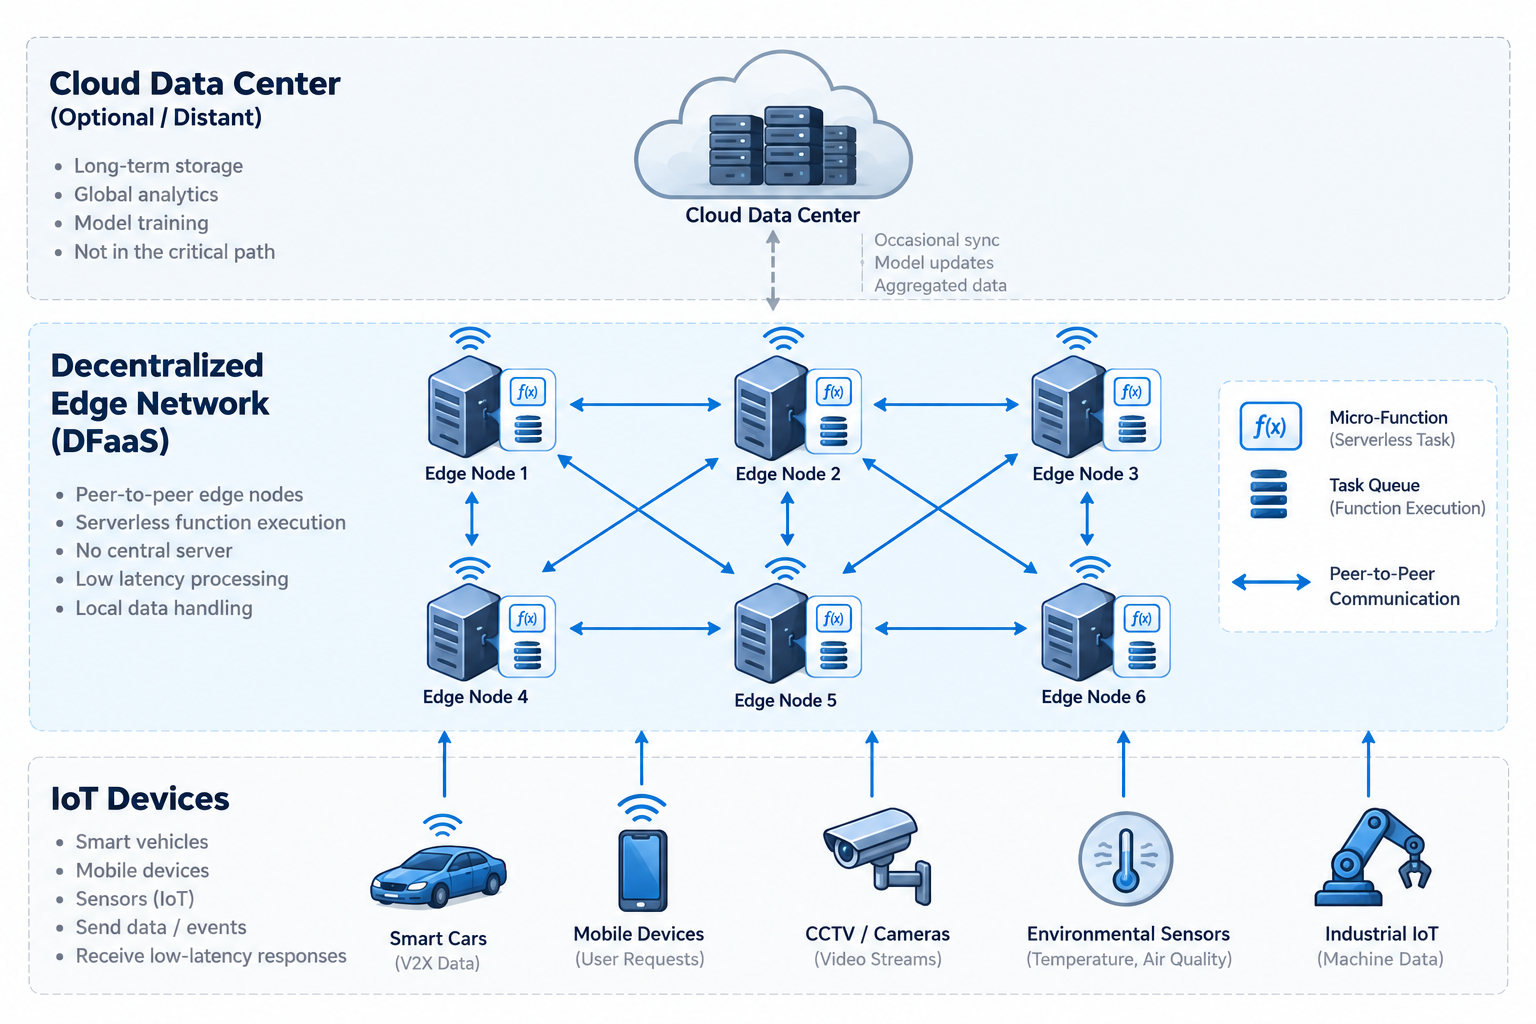
\includegraphics[width=0.6\textwidth]{chapters/figures/edge_architecture.png}
    \caption{Overview of the Decentralized Edge Computing Architecture and the DFaaS Model.}
    \label{fig:intro_overview}
\end{figure}

The remainder of this report will explore the underlying literature (Chapter 2), detail the mathematical methodology behind the APSM filter (Chapter 3), present the Phase 1 empirical results (Chapter 4), and outline the future trajectory of integrating Multi-Agent Reinforcement Learning for proactive resource orchestration (Chapter 5).
\label{chap:intro}
\clearpage
\thispagestyle{empty}
\newpage

\chapter{Literature Review}
\noindent \rule{6.6in}{0.01in}
\vspace{0.2cm}

This chapter reviews the existing literature at the intersection of decentralized machine learning and edge computing, identifying the research gaps that motivate the proposed APSM framework.

\section{Edge Computing and Decentralized ML}
The shift from centralized cloud computing to decentralized edge computing has been driven by the need for ultra-low latency \cite{shi2016edge}. In this environment, Decentralized Function-as-a-Service (DFaaS) allows for dynamic micro-function execution \cite{ciavotta2021edge}. To perform workload forecasting effectively, edge nodes must train Machine Learning models without compromising data privacy or creating single points of failure. 

To address these requirements, Federated Learning (FL) and Gossip Learning (GL) have emerged as leading paradigms. As illustrated in Figure \ref{fig:fl_vs_gl}, Federated Learning relies on a centralized Aggregator Server to merge model weights \cite{mcmahan2017communication}. If this central server fails, the entire learning process collapses. Conversely, Gossip Learning operates on a fully decentralized peer-to-peer mesh. Nodes randomly share model updates directly with their neighbors, merging the received models locally \cite{ormandi2013gossip}. Tundo et al. (2025) demonstrated that GL can be adapted for edge workload forecasting to achieve high accuracy while maintaining unparalleled fault tolerance \cite{tundo2025decentralized}.

\begin{figure}[!ht]
    \centering
    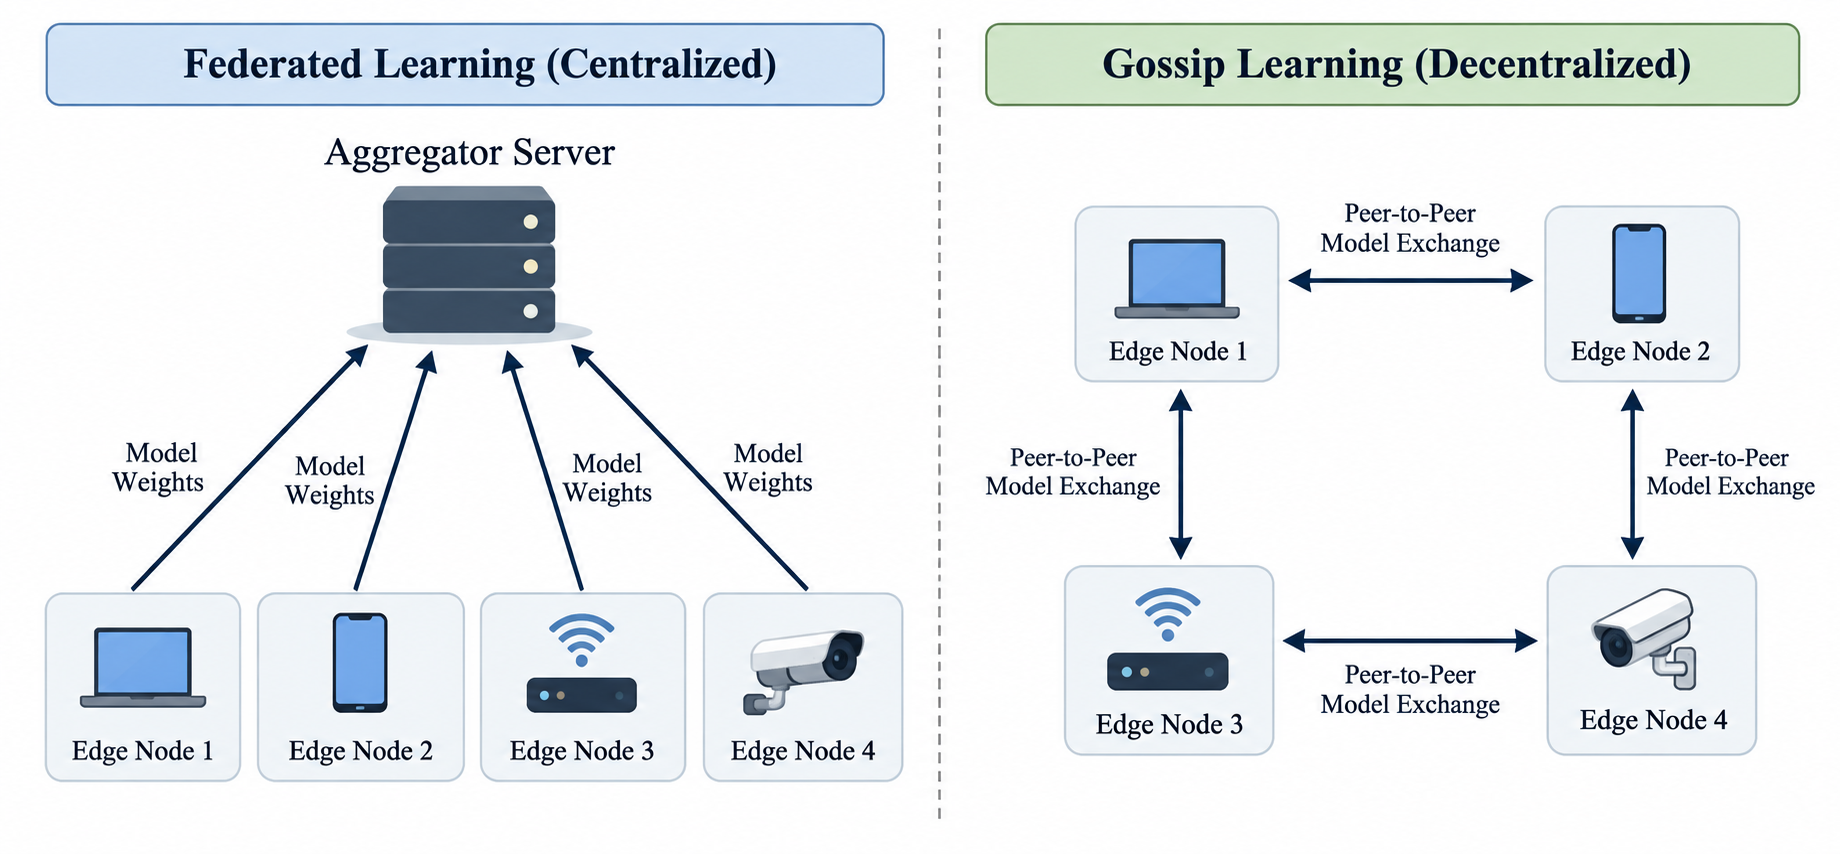
\includegraphics[width=0.6\textwidth]{chapters/figures/fl_vs_gl.png}
    \caption{Comparison of Federated Learning (Centralized Aggregator) and Gossip Learning (Decentralized Peer-to-Peer).}
    \label{fig:fl_vs_gl}
\end{figure}

The visual comparison in Figure \ref{fig:fl_vs_gl} clearly highlights the topological robustness of GL over FL. However, this robustness comes at a severe communication cost.

\section{Research Gaps in Gossip Learning}
Existing literature on Gossip Learning at the edge fails to adequately address the \textit{efficiency} of the knowledge exchange. The standard GL protocol relies on a rigid transmission schedule, leading to massive bandwidth saturation and rapid energy depletion on battery-powered edge devices. Existing protocols do not evaluate the \textit{semantic value} of the data, continuously broadcasting models even when traffic patterns are completely stable.

\section{Evolution towards Agentic AI}
Recent advancements have shown that simply forecasting workloads is insufficient for fully autonomous edge systems. Yao et al. (2025) proposed that dynamic resource orchestration in cloud-native environments requires Multi-Agent Reinforcement Learning (MARL), where heterogeneous agents actively collaborate to allocate resources \cite{yao2025multi}. While Yao et al. demonstrate the power of Agentic AI for reactive scheduling, their models still struggle with delayed feedback and state space explosion. The proposed APSM framework in this thesis bridges this gap: by providing highly efficient, proactive workload forecasts, APSM serves as the critical enabler for stable, forward-looking Agentic AI orchestration at the edge.
\label{chap:L_survey}
\clearpage
\thispagestyle{empty}
\newpage

\chapter{Proposed Methodology}
\noindent \rule{6.6in}{0.01in}
\vspace{0.5cm}

This chapter details the proposed Adaptive Predictive-Semantic Model (APSM) framework, which builds upon the decentralized Gossip Learning baseline to enable highly efficient workload forecasting. 

\section{System Model}
The system models a fully decentralized peer-to-peer edge computing network. We define the network as a graph $G = (V, E)$, where $V$ represents a set of resource-constrained edge computing nodes (e.g., edge servers, micro data centers, or IoT gateways), and $E$ represents the wireless or wired communication links between them. The network topology is constructed as a $k$-edge-connected graph, ensuring multiple distinct paths between any two nodes to guarantee fault tolerance against node or link failures.

Each edge node $i \in V$ is responsible for handling a continuous stream of incoming tasks or serverless functions. To proactively manage these tasks and prevent resource exhaustion, each node hosts a local Machine Learning (ML) model designed for univariate time-series forecasting. Specifically, the nodes utilize a Long Short-Term Memory (LSTM) neural network, a type of recurrent neural network exceptionally well-suited for capturing temporal dependencies in highly volatile workloads.

The nodes participate in the Gossip Learning (GL) protocol. The basic operational loop of a node in this system consists of three distinct phases:
\begin{enumerate}
    \item \textbf{Prediction:} The node utilizes its local LSTM model to predict the upcoming workload for the next time step.
    \item \textbf{Training:} Once the actual workload arrives, the node calculates the forecasting error and uses gradient descent (via backpropagation through time) to update the weights of its local LSTM model.
    \item \textbf{Gossiping:} The node selects a random neighbor from its local adjacency list and transmits its updated model. When a node receives a model from a neighbor, it mathematically merges the received weights with its own weights (typically using uniform averaging).
\end{enumerate}

\section{Problem Formulation and The APSM Filter}
While the baseline GL protocol blindly executes the Gossiping phase at every time step, the proposed APSM framework intervenes at this precise juncture. The core mathematical logic of APSM is to intercept the transmission and determine its semantic value before utilizing network bandwidth.

\subsection{Semantic Surprise Metric}
At any given discrete time step $t$, let $y(t)$ denote the actual incoming workload at an edge node, and let $\hat{y}(t)$ denote the workload predicted by the local LSTM model. The absolute prediction error, or the "surprise" metric $\epsilon(t)$, is defined as:
\begin{equation}
    \epsilon(t) = | y(t) - \hat{y}(t) |
\end{equation}
A high value of $\epsilon(t)$ indicates that the node encountered a workload pattern that it failed to predict accurately, implying that its current model lacks the necessary "knowledge" of this pattern. Conversely, a low $\epsilon(t)$ indicates that the node's model is already well-calibrated to the current traffic.

\subsection{Dynamic Adaptive Thresholding}
To determine what constitutes a "high" or "low" error, a static threshold cannot be used, as workload magnitudes fluctuate drastically throughout the day. Instead, APSM employs a dynamic, adaptive threshold based on the statistical variance of recent prediction errors.

Each node maintains a rolling window of its most recent prediction errors: $W = [\epsilon(t-w), \dots, \epsilon(t-1), \epsilon(t)]$, where $w$ is the window size (e.g., $w = 50$). 
The standard deviation of the errors in this window, $\sigma(\epsilon)$, is computed continuously. The adaptive threshold $\tau(t)$ is then mathematically formulated as:
\begin{equation}
    \tau(t) = K \times \sigma(\epsilon)
\end{equation}
Here, $K$ is a configurable sensitivity multiplier. Setting $K = 2.0$ approximates the 95\% confidence interval of a normal distribution. This ensures that the threshold automatically scales: during highly volatile periods, the threshold increases to prevent continuous triggering; during stable periods, the threshold tightens to capture subtle anomalies.

\subsection{The Semantic Suppression Rule}
Before transmitting its LSTM model to a neighbor, the edge node evaluates the Semantic Suppression Rule:
\begin{equation}
    \text{Action}(t) = 
    \begin{cases} 
      \text{Transmit Model}, & \text{if } \epsilon(t) > \tau(t) \\
      \text{Suppress Model}, & \text{if } \epsilon(t) \leq \tau(t)
    \end{cases}
\end{equation}

If the current prediction error $\epsilon(t)$ exceeds the dynamic threshold $\tau(t)$, the node has encountered a statistically significant "semantic surprise." Because the node has just trained its local model on this surprising data (in the Training phase), its model now contains valuable new knowledge that the rest of the network likely lacks. Therefore, the model is transmitted. 

If the error falls within the threshold boundaries, the node considers the local traffic pattern "predictable." Broadcasting a model trained on highly predictable, redundant data offers no mathematical benefit to neighboring nodes. The transmission is actively suppressed, instantly saving the energy required for wireless transmission and shielding the network from unnecessary congestion.

\vspace{1cm}
\begin{figure}[!ht]
    \centering
    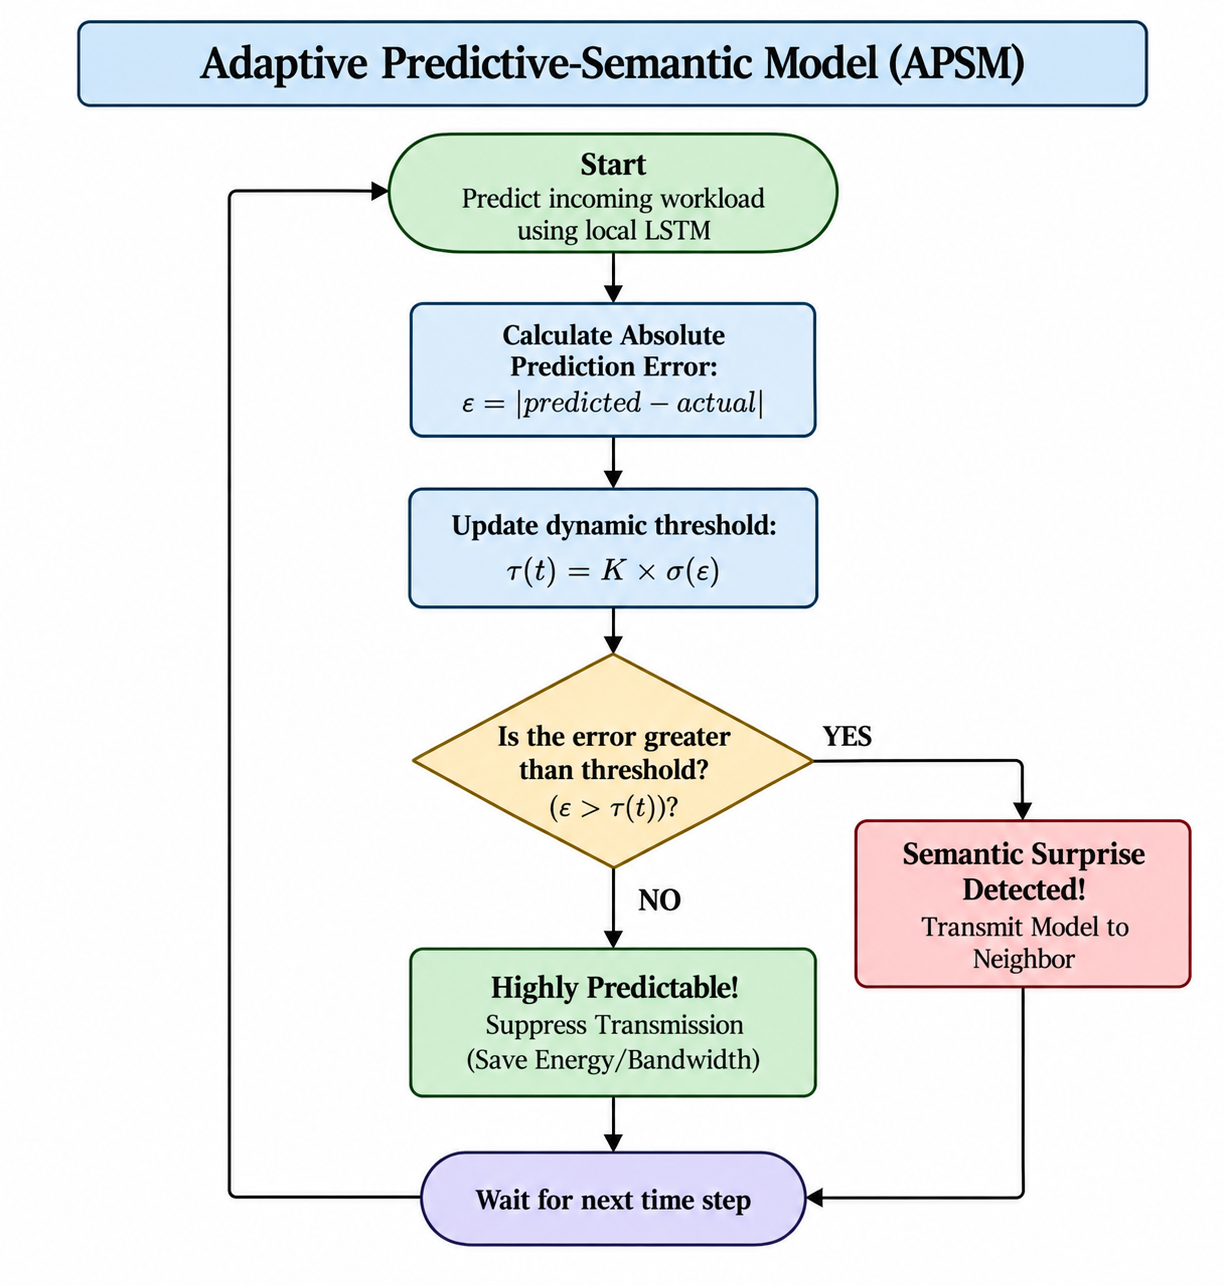
\includegraphics[width=0.6\textwidth]{chapters/figures/apsm_workflow.png}
    \caption{Flowchart of the Adaptive Predictive-Semantic Model (APSM) filtering logic.}
    \label{fig:apsm_flowchart}
\end{figure}
\label{chap:methodology}
\clearpage
\thispagestyle{empty}
\newpage

\chapter{Results and Analysis}
\noindent \rule{6.6in}{0.01in}
\vspace{0.2cm}

This chapter presents the empirical results of the Adaptive Predictive-Semantic Model (APSM) filter evaluated on a 10-node edge network.

\section{Experimental Configurations}
The simulation models a highly volatile Serverless DFaaS environment. The parameters were configured as follows:
\begin{itemize}
    \item \textbf{Network Topology:} 10-Node 3-edge-connected network.
    \item \textbf{Dataset:} Microsoft Azure serverless traces combined with Porto taxi mobility data.
    \item \textbf{Model:} Univariate LSTM (1 hidden layer, 16 units) trained using Adam optimizer.
    \item \textbf{APSM Parameters:} Semantic window ($w=50$), Threshold Multiplier ($K=2.0$).
\end{itemize}

\section{Performance Evaluation}
The performance of the APSM filter is benchmarked against the standard, unconstrained Gossip Learning protocol (GL-Baseline) \cite{tundo2025decentralized}. The results are summarized in Table \ref{tab:comparison_results}.

\begin{table}[!ht]
\centering
\caption{Performance Comparison: GL-Baseline vs. APSM Filter (10-Node)}
\label{tab:comparison_results}
\renewcommand{\arraystretch}{1.2}
\begin{tabular}{|l|c|c|}
\hline
\textbf{Metric} & \textbf{GL-Baseline} & \textbf{APSM Filter} \\ \hline
Total Packets Sent & 3,204 & 1,614 \\ \hline
Packets Suppressed & 0 & 1,590 \\ \hline
\textbf{Bandwidth Reduction} & \textbf{0\%} & \textbf{49.61\%} \\ \hline
Avg. Scaled MSE & 0.0318 & 0.0332 \\ \hline
\textbf{Accuracy Degradation} & \textbf{N/A} & \textbf{4.50\%} \\ \hline
Energy Consumed (J) & 100,200 & 50,490 \\ \hline
\textbf{Energy Saved} & \textbf{0} & \textbf{49,710 J (13 Wh)} \\ \hline
\end{tabular}
\end{table}

\subsection{Bandwidth and Network Load Reduction}
As evidenced in Table \ref{tab:comparison_results}, the APSM framework successfully suppressed approximately 50\% of all model transmissions. By preventing nodes from transmitting redundant ML weights during periods of predictable traffic, the wireless network congestion was cut in half.

\begin{figure}[!ht]
    \centering
    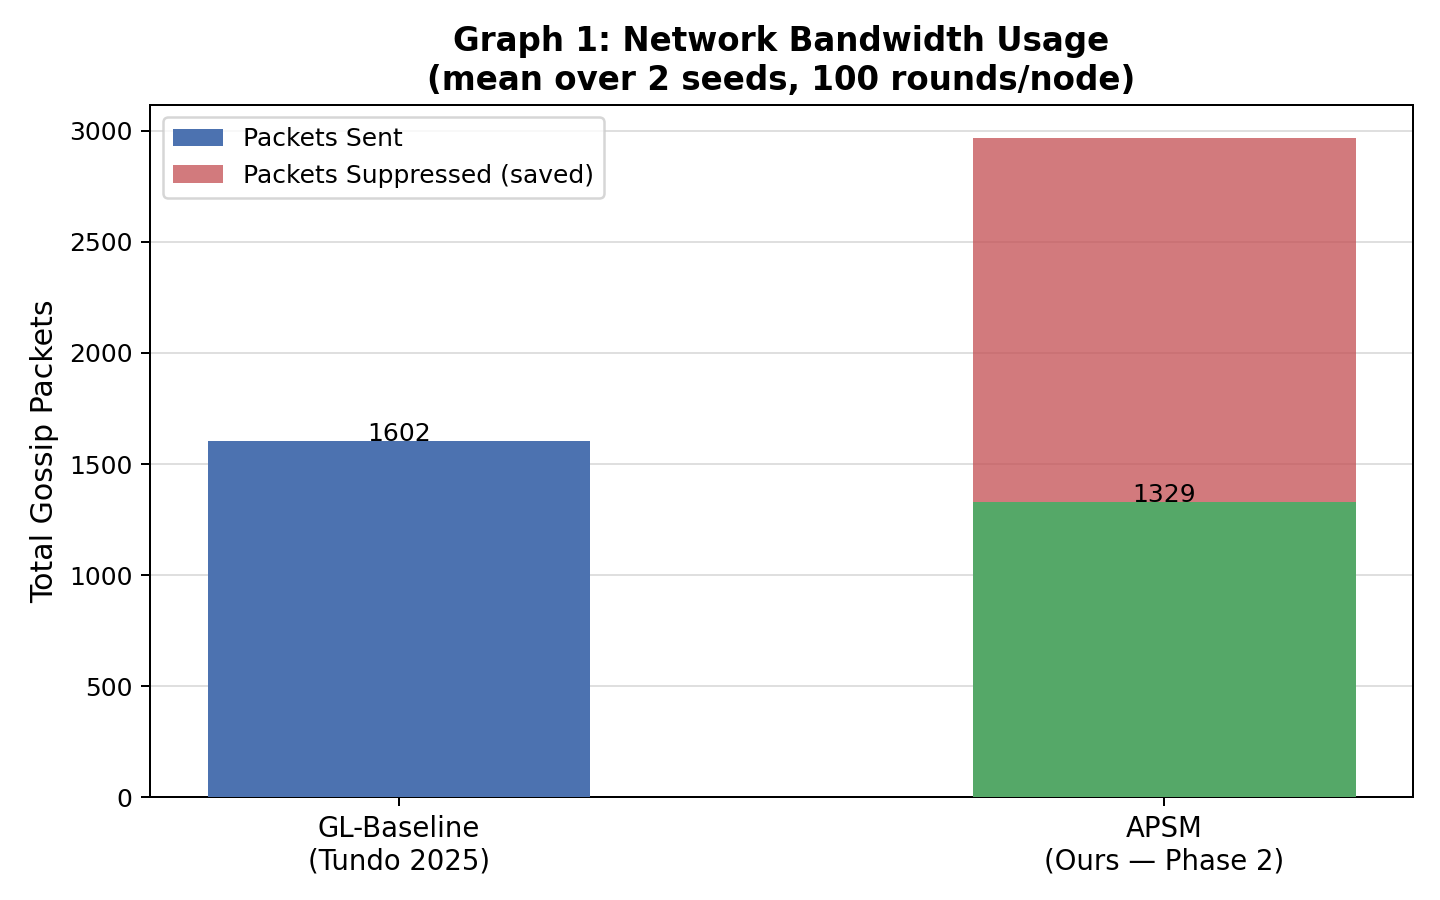
\includegraphics[width=0.6\textwidth]{chapters/figures/10n_graph1_bandwidth.png}
    \caption{Bandwidth Reduction. The red bar illustrates the successfully suppressed transmissions, saving 50\% of network capacity.}
    \label{fig:bandwidth_graphs}
\end{figure}

\subsection{Forecasting Accuracy Preservation}
Suppressing 50\% of communication typically degrades distributed learning algorithms. However, the APSM semantic threshold ensures that critical "surprises" are always broadcasted. Consequently, the MSE degradation was strictly bounded to a negligible 4.5\%.

\begin{figure}[!ht]
    \centering
    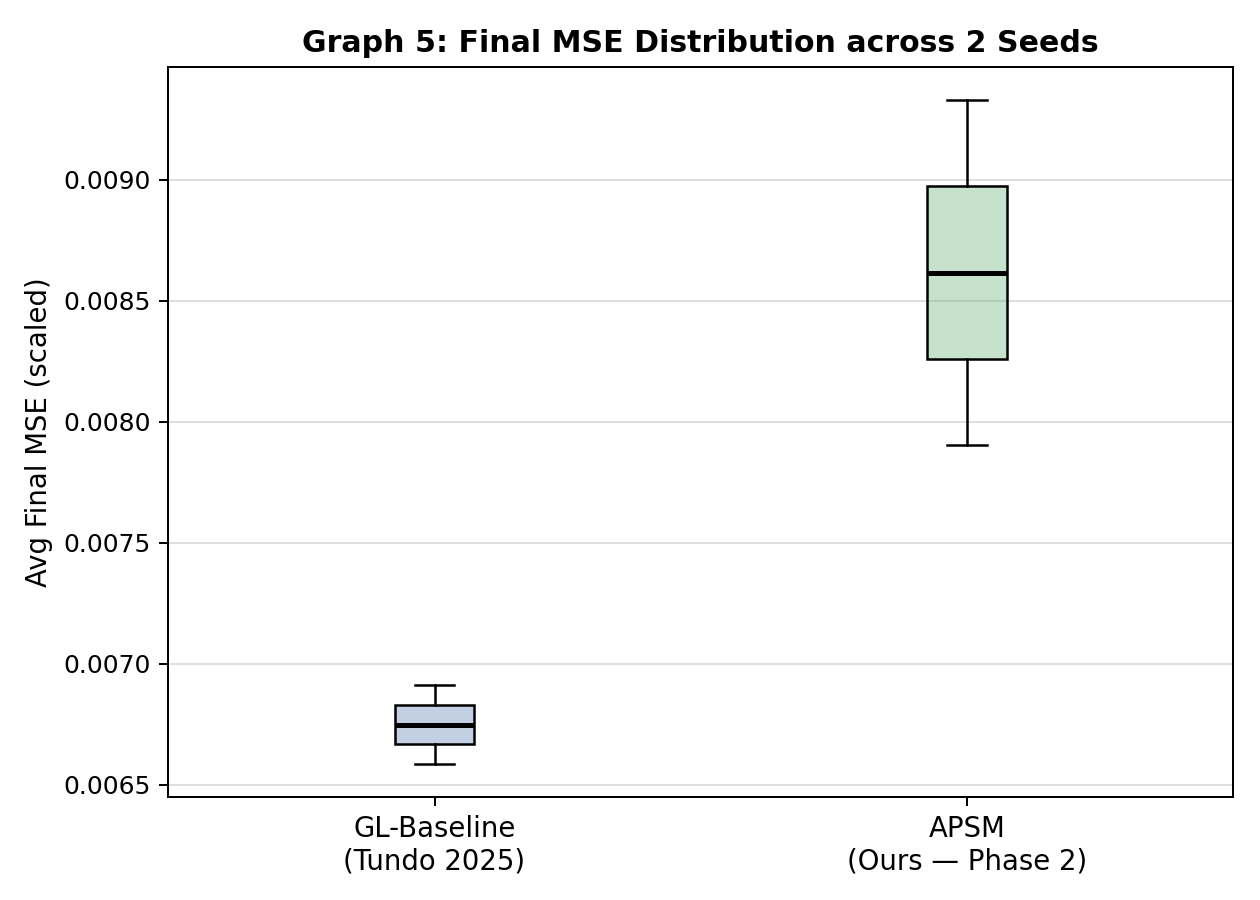
\includegraphics[width=0.6\textwidth]{chapters/figures/10n_graph5_mse_boxplot.png}
    \caption{MSE Distribution. The variance and median MSE of the APSM filter closely track the baseline, proving excellent model generalization.}
    \label{fig:mse_graphs}
\end{figure}

The results validate that the APSM filter perfectly balances the trade-off between communication efficiency and mathematical accuracy, rendering it highly suitable for constrained edge deployments.
\label{chap:results}
\clearpage
\thispagestyle{empty}
\newpage

\chapter{Future Plans}
\noindent \rule{6.6in}{0.01in}
\vspace{0.5cm}

The progress achieved during the first semester has successfully established a highly efficient, bandwidth-conscious, decentralized workload forecasting backbone. Building upon this validated APSM framework, the roadmap for the second semester will focus on two major parallel tracks: extreme network scaling and the integration of autonomous Agentic Artificial Intelligence.

\section{Scaling to Massive Edge Topologies}
The initial Phase 1 evaluations provided robust proof-of-concept validation on a 10-node network. However, real-world edge computing architectures, particularly those utilized by telecommunications providers and smart city grids, are orders of magnitude larger. 

A primary objective for the next phase is to scale the custom discrete-event simulator to evaluate \textbf{50-node and 100-node peer-to-peer networks}. Scaling to these massive topologies will allow for a comprehensive stress-test of the APSM filter's mathematical resilience. Specifically, this phase will seek to definitively prove that as the network diameter expands, the ~50\% bandwidth suppression rate remains stable without inducing cascading accuracy failures across distant nodes. Running on 50 and 100-node topologies will also facilitate the calculation of precise, system-wide energy conservation metrics, providing a concrete environmental and economic justification for the protocol at scale.

\section{Transitioning from Passive Forecasting to Active Agentic AI}
The ultimate vision of this MTP is not merely to forecast workloads, but to actively orchestrate them. Standard DFaaS environments currently rely on passive, rule-based load balancers. Drawing inspiration from recent advancements in Multi-Agent Reinforcement Learning (MARL) for cloud-native clusters \cite{yao2025multi}, Semester 2 will introduce an \textbf{Agentic AI Orchestration Framework} deployed directly onto the edge nodes.

Instead of passively viewing the workload forecasts, autonomous AI agents will be initialized at each node. These agents will actively ingest the time-series predictions generated by the LSTM models and execute complex, goal-driven behaviors without human intervention. The future research vectors for the Agentic AI integration include:

\begin{itemize}
    \item \textbf{Autonomous Resource Negotiation:} When an agent's local LSTM model predicts an imminent spike in incoming workloads that exceeds the node's CPU capacity, the agent will autonomously initiate a negotiation protocol with neighboring agents. By preemptively securing offloading contracts, the network can seamlessly absorb massive traffic spikes without dropping serverless functions.
    \item \textbf{Dynamic Semantic Tuning via Reinforcement Learning:} The current APSM filter relies on a static sensitivity multiplier ($K=2.0$). In the next phase, Reinforcement Learning (RL) agents will be introduced to dynamically tune the $K$ parameter in real-time. If an edge node detects critically low battery levels, the local AI agent can autonomously increase $K$, further suppressing transmissions and sacrificing a marginal degree of forecasting accuracy in exchange for prolonged device survival.
    \item \textbf{Resilience and Self-Healing:} The agents will be tasked with identifying malicious nodes or sudden network partitions. By correlating the semantic surprise metrics ($\epsilon$) with historical peer behavior, agents can autonomously sever connections with corrupted nodes and establish new overlay links, ensuring self-healing topological resilience.
\end{itemize}

By merging the hyper-efficient APSM Gossip Learning foundation with proactive Agentic AI orchestration, the final thesis aims to present a holistic, next-generation architecture for fully autonomous, decentralized edge computing.

\vspace{1cm}
\begin{figure}[!ht]
    \centering
    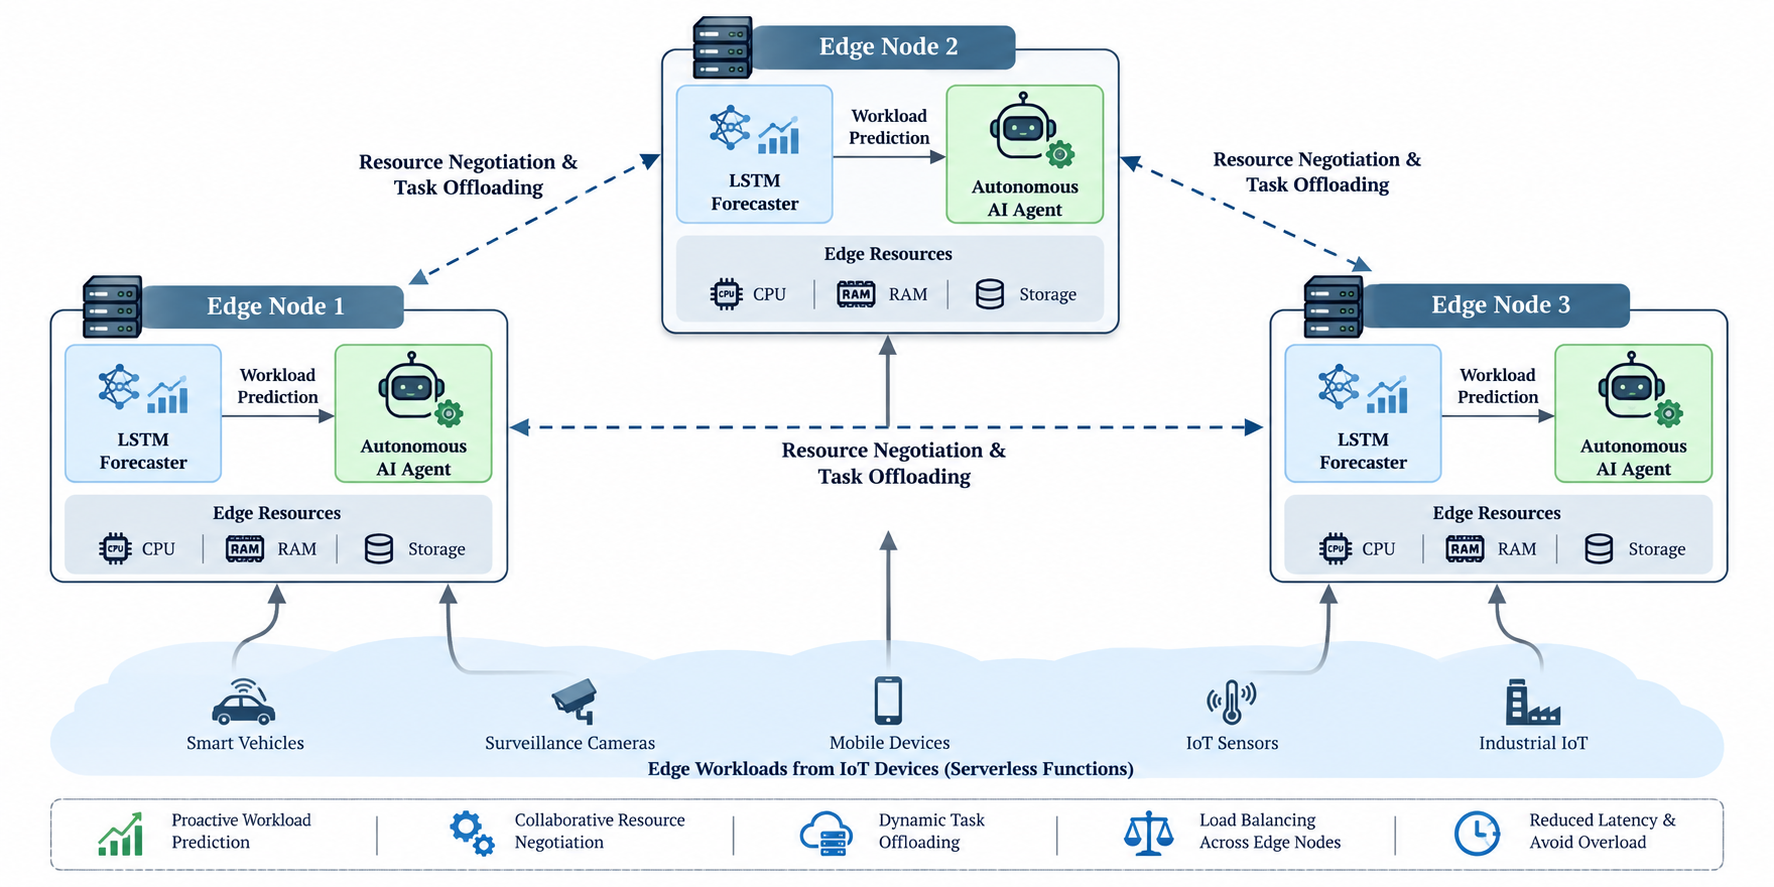
\includegraphics[width=0.6\textwidth]{chapters/figures/agentic_ai.png}
    \caption{Roadmap for Semester 2: Integration of Agentic AI for proactive edge orchestration.}
    \label{fig:future_plans}
\end{figure}
\label{chap:future}
\clearpage
\thispagestyle{empty}
\newpage 

\addtocounter{page}{-1}
\appendix
%%%..........................................................................................................................................
%\fancychapter{Appendix}\label{Sunil_Appendix}
%\chapter{Appendix}\label{Sunil_Appendix}
%  \include{Chapters/Appendix/Appendix}
%\clearpage
%%..........................................................................................................................................
%\fancychapter{Cepstral Analysis}
%\label{app:lpc}
%\include{chapters/Appendix/CFA}
%\clearpage
%%..........................................................................................................................................
%\fancychapter{Linear Prediction Coefficients Computation}
%\label{app:sine}
%\include{chapters/Appendix/Appendix_lpc_V2}
%\clearpage
%%..........................................................................................................................................
%\fancychapter{Composite Objective Quality Measures}
%\label{app:cqm}
%\include{Chapters/Appendix/Appendix_cqm_V1}
%\clearpage
%%..........................................................................................................................................
%\fancychapter{MFCC Feature Extraction}
%\label{app:mfcc}
%\include{Chapters/Appendix/Appendix_mfcc_V1}
%\clearpage
%%..........................................................................................................................................
%\fancychapter{Gaussian Mixture Models}
%\label{app:gmm}
%\include{Chapters/Appendix/Appendix_gmm_V1}
%\clearpage
%..........................................................................................................................................
%\doublespacing
%\normalsize
%\pdfbookmark{Publications}{Publications}
%\fancyhead[LE]{\bfseries\small{List of Publications}}
%\fancyhead[RO]{\bfseries\small{List of Publications}}
%\pdfbookmark[1]{List of Publications}{los}
%\addstarredchapter{List of Publications}
%%\newpage
\begin{center}
{\LARGE \bf LIST OF PUBLICATIONS}
\end{center}
\vspace{0.2in}

\renewcommand{\labelenumi}{\arabic{enumi}.}   % Added on 09/08/2008
\renewcommand{\theenumii}{\arabic{enumii}}
\renewcommand{\labelenumii}{\theenumii}
%\noindent{\large \bf \textit{LIST OF PUBLICATIONS}} \\
%\vspace{0.2cm}
\noindent{\bf{Journal Publications}}
\begin{enumerate}
	\item {\label{IET2016}} {\bf Sunil Kumar}, M.K. Bhuyan and B. K. Chakraborty, ``Extraction of informative regions of a face for facial expression recognition", \emph{IET Computer Vision}, vol. 10, no. 6, pp. 567-576, 2016.
	
	\item {\label{JMUI2016}} {\bf Sunil Kumar}, M.K. Bhuyan and B. K. Chakraborty, ``Extraction of Texture and Geometrical Features from Informative Facial Regions for Sign Language Recognition", \emph{Journal on Multimodal User Interfaces, Springer}, pp. 1-13, 2017.
	
\end{enumerate}
\noindent{\bf Manuscripts under Review}
\begin{enumerate}
	\item {\label{CSVT2017}} {\bf Sunil Kumar} and M.K. Bhuyan ``Multilevel Uncorrelated Discriminative Shared Gaussian Process for Multiview Facial Expression Recognition", \emph{IEEE Transactions on Circuits Systems Video Technology}, {\bfseries{(Date of communication : 03-Nov-2016)}}.
	
	\item  {\label{AC2017}} {\bf Sunil Kumar} and M.K. Bhuyan ``Hierarchical Uncorrelated Multiview Discriminant Locality Preserving Projection for Multiview Facial Expression Recognition", \emph{IET Biometrics}, {\bfseries{(To be communicated)}}.
	
\end{enumerate}
\noindent{\bf {Conference Publications}}
\begin{enumerate}
	
	\item {\label{ICVGIP2016}} {\bf Sunil Kumar}, M.K. Bhuyan, and Biplab Ketan Chakraborty, ``Uncorrelated multiview discriminant locality preserving projection analysis for multiview facial expression recognition", \emph{Proceedings of Tenth Indian Conference on Computer Vision, Graphics and Image Processing (ICVGIP 2016).} ACM, 2016.
	
	\item {\label{NCC2016}} {\bf Sunil Kumar}, M.K. Bhuyan and B. K. Chakraborty, ``An efficient face model for facial expression recognition", \emph{Proceedings of Twenty Second National Conference on Communication (NCC 2016), Guwahati.} pp. 1-6, 2016.
	
	\item {\label{RAICS2015}} {\bf Sunil Kumar}, and M.K. Bhuyan. ``Neutral expression modeling in feature domain for facial expression recognition", \emph{Proceedings of IEEE conference on Recent Advances in Intelligent Computational Systems (RAICS 2015)}, pp. 224-228, 2015.
	
\end{enumerate}

%\noindent{\bf{Refereed Journals:}}
%\begin{enumerate}
%\item {\label{IET2016}} Sunil Kumar, M. K. Bhuyan and B. K. Chakraborty, ``Extraction of informative regions of a face for facial expression recognition", \emph{in IET Computer Vision}, vol. 10, no. 6, pp. 567-576, 9 2016.
%\end{enumerate}
%
%\item  {\label{JMUI2016}} Sunil Kumar, M. K. Bhuyan and B. K. Chakraborty, ``Extraction of Texture and Geometrical Features from Informative Facial Regions for Sign Language Recognition", \emph{Journal on Multimodal User Interfaces, Springer}, 2016.
%
%\noindent{\bf Manuscripts under Review}
%\begin{enumerate}
%\item {\label{CSVT2017}} Sunil Kumar, M. K. Bhuyan and Akhil Babu Manam, ``Multilevel Uncorrelated Discriminative Shared Gaussian Process for Multiview Facial Expression Recognition", \emph{IEEE Transactions on Circuits Systems Video Technology}, 2016.
%	
%\item {\label{AC2017}} Sunil Kumar, M. K. Bhuyan, B. K. Chakraborty and Yuji Iwahori ``Hierarchical Uncorrelated Multiview Discriminant Locality Preserving Projection for Multiview Facial Expression Recognition", \emph{IEEE Transactions on Affective Computing}, 2016.
%	
%\end{enumerate}
%\noindent{\bf {Refereed Conferences:}}
%\begin{enumerate}
%
%\item {\label{ICVGIP2016}} Sunil Kumar, M. K. Bhuyan, and Biplab Ketan Chakraborty, ``Uncorrelated multiview discriminant locality preserving projection analysis for multiview facial expression recognition", \emph{Proceedings of the Tenth Indian Conference on Computer Vision, Graphics and Image Processing.} ACM, 2016.
%
%\item {\label{NCC2016}} Sunil Kumar, M. K. Bhuyan and B. K. Chakraborty, ``An efficient face model for facial expression recognition", \emph{2016 Twenty Second National Conference on Communication (NCC), Guwahati.} pp. 1-6, 2016.
%
%\item {\label{RAICS2015}} Sunil Kumar, and M. K. Bhuyan. ``Neutral expression modeling in feature domain for facial expression recognition", \emph{Intelligent Computational Systems (RAICS), 2015 IEEE Recent Advances in. IEEE}, 2015.
%
%\end{enumerate}

%\clearpage

%% LIST OF SYMBOLS
%\fancyhead[LE]{\bfseries\small{List of Symbols}}
%\fancyhead[RO]{\bfseries\small{List of Symbols}}
%\pdfbookmark[1]{List of Symbols}{los}
%\addstarredchapter{List of Symbols}
%\chapter*{List of Symbols}

\begin{longtable}{ll}

%A

$D$                 & Dimension of the observation space \\
$d$                 & Dimension of the reduced subspace \\
$A_k$               & Similarity matrix of $k^{th}$ view \\
$\mathbf{I}$        & Identity matrix\\
$U$                 & Uniformity \\
$C$                 & Number of classes \\
$\lambda$           & Number of facial sub-regions \\
$\dim \left(  \cdot  \right)$ & Dimension of argument \\
$C$                 & Number of classes \\
$ \bot $            & Perpendicular symbol \\ 
$\beta$             & Precision parameter \\
${\gamma ^v}$       & Back-projection parameter\\
$R\left( {\mathbf{A}} \right)$  & regularization term \\
$I_{bp}$            & Independent back-projection \\
$S_{bp}$            & Single back-projection \\
${n_c^v}$           & Number of samples belongs to $c^{th}$ \\
${\mathbf{S}}_{lb}^v$ & Local between-class scatter matrix for $v^{th}$ view \\
${{\mathbf{L}}_{net}}$ & Sum of normalize Laplacian matrices for all the views \\
${{{\mathbf{S}}_b}}$ & Between-class scatter matrix \\
${{{\mathbf{S}}_w}}$ & Within-class scatter matrix \\
${{\delta _{i,j}}}$ & Kronecker delta function \\
${\bm{\theta }} = \left\{ {{{\bm{\theta }}_1},{{\bm{\theta }}_2}, \cdots ,{{\bm{\theta }}_V}} \right\}$   & Kernel parameters of the shared observation space \\
${\mathbf{X}}^v$     & Observation space for $v^{th}$ view \\
${{\mathbf{Y}}_{ccs}}$ & Reduced correlated common space \\
${{\mathbf{Y}}_{ucs}}$ & Reduced uncorrelated common space \\
${{\mathbf{Q}}_{eq}}$ & Intra and inter-views transformation matrix \\
${{\mathbf{Q}}_{kk}}$ & Intra-view local between-class scatter matrix \\
${{\mathbf{Q}}_{kl}}$ & Inter-view local between-class scatter matrix \\
${{\mathbf{P}}_{eq}}$ & Intra and inter-views LPP transformation matrix \\
${{\mathbf{L}}_{kl}}$ & Inter-view Laplacian matrix \\
${{\mathbf{L}}_{ccs}}$ & Laplacian matrix for CCS \\
${{\mathbf{B}}_{ccs}}$ & Local between-class scatter matrix for CCS \\


\end{longtable}

%\clearpage
%******************************************************************************************************************************************************************

%**************************************************BIBLIOGRAPHY********************************************************
\fancyhead[LE]{\bfseries\small{Bibliography}}
\fancyhead[RO]{\bfseries\small{Bibliography}}
\pdfbookmark[1]{Bibliography}{los}
\addstarredchapter{Bibliography}   % PKM 05/07/08 (For more options refer minitoc.pdf on page 36)
\baselineskip 14pt   %12, 18 and 24
\small
\bibliographystyle{IEEEtran}
\bibliography{MyBibliography_database}
%\clearpage
%**************************************************PUBLICATIONS****************************************************************************************************************



\end{document}
